\documentclass[10pt, aspectratio=169]{beamer}

\usepackage[utf8]{inputenc}
\usepackage[T1]{fontenc}
\usepackage[french]{babel}
\usepackage{lmodern}
\usepackage{graphicx}
\usepackage{booktabs}
\usepackage{amsmath}
\usepackage{caption}

% Thème
\usetheme{Boadilla}
\usecolortheme{seahorse}
\setbeamertemplate{navigation symbols}{} % Supprimer les symboles de navigation

% Définition de couleurs personnalisées pour rappeler le rapport
\definecolor{stormblue}{HTML}{0B1F33}
\definecolor{rainblue}{HTML}{1F77B4}
\setbeamercolor{structure}{fg=stormblue}
\setbeamercolor{title}{fg=stormblue}
\setbeamercolor{frametitle}{fg=stormblue}
\setbeamercolor{itemize item}{fg=rainblue}
\setbeamercolor{itemize subitem}{fg=rainblue}

\title[Génération d'extrêmes climatiques]{Génération de champs de précipitations extrêmes en France}
\subtitle{Comparaison entre VAE, GAN et WGAN-GP}
\author[Projet GenAI]{
    \begin{tabular}{rl}
        \textbf{Auteurs :} & Nom Prénom 1 \\
                           & Nom Prénom 2 \\
                           & Nom Prénom 3 \\[0.3em]
        \textbf{Encadrant :} & Nom Prénom
    \end{tabular}
}
\institute[ENSAE]{ENSAE Paris}
\date{27 avril 2026}

\begin{document}

% Slide 1 : Titre
\begin{frame}
    \titlepage
\end{frame}

% Slide 2 : Introduction
\begin{frame}{Introduction \& Enjeux}
    \textbf{Le problème :}
    \begin{itemize}
        \item Évaluer les risques climatiques (inondations, infrastructures) nécessite d'explorer la \textbf{queue de distribution} des événements rares.
        \item Les Modèles de Circulation Générale (GCM) sont physiquement robustes mais \textbf{trop lents et coûteux} pour générer de très grands ensembles.
    \end{itemize}
    \vspace{0.5cm}
    \textbf{Notre objectif :}
    \begin{itemize}
        \item Évaluer les \textbf{Modèles Génératifs Profonds (DGM)} comme émulateurs climatiques stochastiques rapides.
        \item Cible : Générer l'indice \textbf{Rx5day} (précipitation maximale sur 5 jours consécutifs).
        \item Défi : Reproduire la structure spatiale, l'asymétrie statistique et les contrastes régionaux.
    \end{itemize}
\end{frame}

% Slide 3 : Données
\begin{frame}{Données et Prétraitement}
    \begin{columns}
        \begin{column}{0.55\textwidth}
            \textbf{Source des données :}
            \begin{itemize}
                \item Copernicus CDS : projections globales \textbf{CMIP6} [1, 2].
                \item Fenêtre spatiale : France métropolitaine ($8 \times 10$ pixels).
            \end{itemize}
            \vspace{0.3cm}
            \textbf{Le défi du Min-Max Scaling :}
            \begin{itemize}
                \item Normalisation vers $[0, 1]$ obligatoire pour les réseaux de neurones (activations sigmoïdes).
                \item \textbf{Problème :} Les extrêmes suivent une loi à queue lourde. Le scaling écrase la vaste majorité des valeurs près de 0.
                \item \textbf{Conséquence :} L'apprentissage de la différence entre pluie modérée et tempête extrême devient numériquement très difficile.
            \end{itemize}
        \end{column}
        \begin{column}{0.45\textwidth}
            \centering
            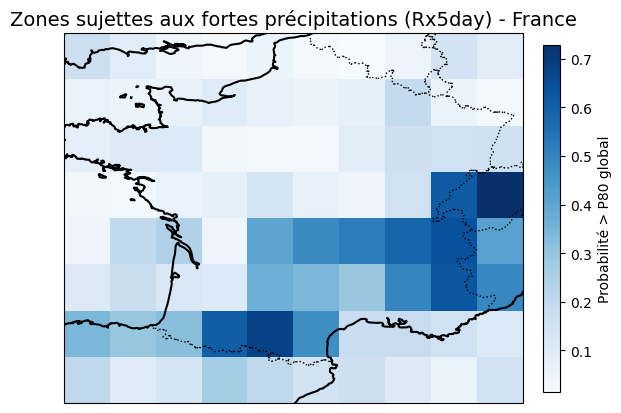
\includegraphics[width=0.9\textwidth]{../images/EDA/heavy_precipitation_probability_map.png}
            \captionof*{figure}{\scriptsize Probabilité empirique de fortes précipitations (P80)}
        \end{column}
    \end{columns}
\end{frame}

% Slide 4 : EDA 1
\begin{frame}{Analyse Exploratoire : Saisonnalité et Asymétrie}
    \begin{columns}
        \begin{column}{0.5\textwidth}
            \centering
            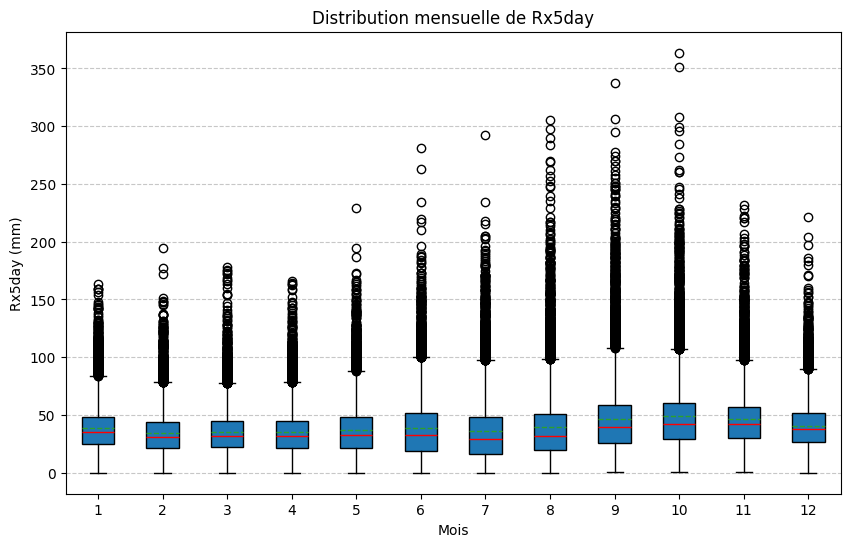
\includegraphics[width=\textwidth]{../images/EDA/monthly_rx5day_boxplot.png}
        \end{column}
        \begin{column}{0.5\textwidth}
            \textbf{Observations clés :}
            \begin{itemize}
                \item \textbf{Forte saisonnalité} : Les mois d'automne et d'hiver concentrent les événements les plus intenses.
                \item \textbf{Asymétrie marquée} : Présence de queues droites très longues (événements extrêmes rares).
                \item Les modèles (VAE/GAN) sont entraînés \textit{sans} conditionnement temporel : ils doivent encoder cette diversité saisonnière de manière non supervisée dans leur espace latent.
            \end{itemize}
        \end{column}
    \end{columns}
\end{frame}

% Slide 5 : EDA 2
\begin{frame}{Analyse Exploratoire : Structure Spatiale}
    \begin{columns}
        \begin{column}{0.5\textwidth}
            \centering
            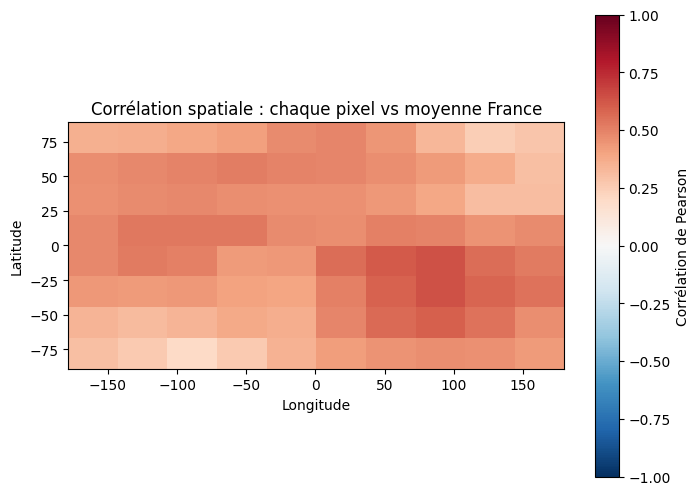
\includegraphics[width=0.75\textwidth]{../images/EDA/spatial_correlation_map.png}
            
            \vspace{0.3cm}
            
            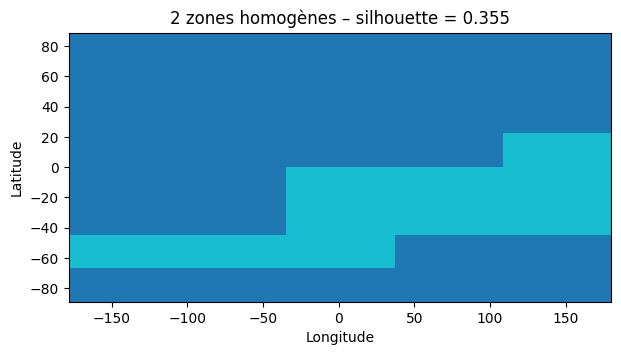
\includegraphics[width=0.75\textwidth]{../images/EDA/homogeneous_precipitation_zones.png}
        \end{column}
        \begin{column}{0.5\textwidth}
            \textbf{Corrélation Spatiale (Haut) :}
            \begin{itemize}
                \item Les pixels voisins réagissent de manière cohérente.
                \item Justifie l'utilisation d'architectures \textbf{CNN} (Réseaux Convolutifs) pour capter les gradients locaux.
            \end{itemize}
            \vspace{0.4cm}
            \textbf{Segmentation K-means (Bas) :}
            \begin{itemize}
                \item Séparation en 2 zones climatiques nettes.
                \item \textbf{Zone 0} : Influence atlantique (fréquent, modéré).
                \item \textbf{Zone 1} : Influence méditerranéenne/reliefs (sporadique, extrême, ex: épisodes cévenols).
            \end{itemize}
        \end{column}
    \end{columns}
\end{frame}

% Slide 6 : EDA 3
\begin{frame}{Analyse Exploratoire : Distribution par Zone}
    \centering
    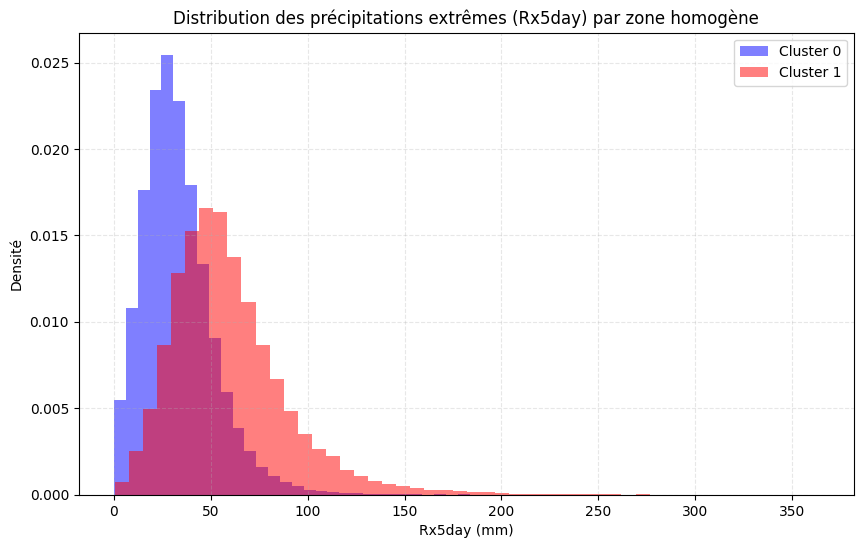
\includegraphics[width=0.7\textwidth]{../images/EDA/cluster_precipitation_distribution.png}
    \captionof*{figure}{\scriptsize Densité des précipitations extrêmes (Rx5day) par zone climatique.}
    \vspace{0.3cm}
    \begin{itemize}
        \item \textbf{Zones d'influence} : Les modèles génératifs devront apprendre à déclencher des motifs d'intensité variable selon les coordonnées spatiales, s'adaptant ainsi à la dualité observée.
    \end{itemize}
\end{frame}

% Slide 7 : VAE
\begin{frame}{Autoencodeur Variationnel (VAE) [3]}
    \begin{columns}
        \begin{column}{0.55\textwidth}
            \textbf{Architecture :}
            \begin{itemize}
                \item Encodeur CNN $\rightarrow$ Espace latent ($dim=8$) $\rightarrow$ Décodeur CNN.
                \item Approche probabiliste : le modèle apprend une distribution continue.
            \end{itemize}
            \vspace{0.3cm}
            \textbf{Fonction de Perte (ELBO) :}
            \[ \mathcal{L} = \underbrace{\lambda_{\mathrm{rec}}\mathcal{L}_{\mathrm{BCE}}}_{\text{Reconstruction}} + \underbrace{\lambda_{\mathrm{KL}}D_{\mathrm{KL}}(q(z|x)\Vert p(z))}_{\text{Régularisation}} \]
            \begin{itemize}
                \item Poids $\lambda_{\mathrm{KL}}$ optimal très faible ($0.005$) pour éviter le \textit{posterior collapse} et forcer la reconstruction détaillée.
            \end{itemize}
        \end{column}
        \begin{column}{0.45\textwidth}
            \centering
            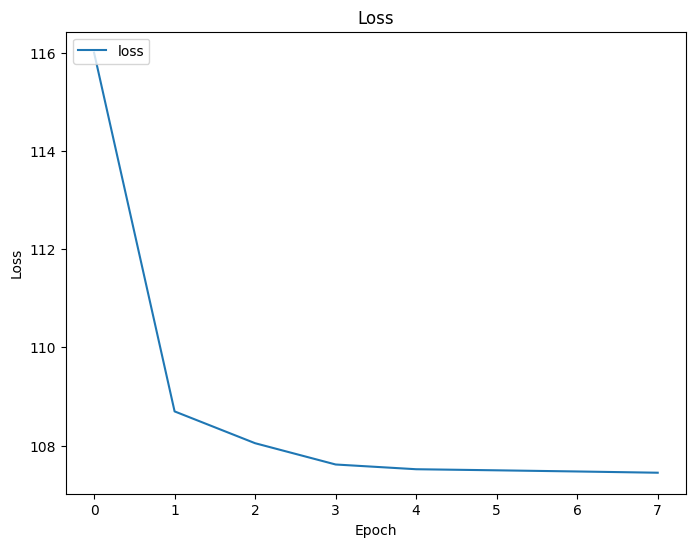
\includegraphics[width=\textwidth]{../images/VAE/vae_training_loss_curve.png}
            \captionof*{figure}{\scriptsize Convergence stable du VAE}
        \end{column}
    \end{columns}
\end{frame}

% Slide 7 : VAE Batch Size
\begin{frame}{Le défi du VAE : L'importance cruciale du Batch Size}
    \textbf{Découverte expérimentale majeure :}
    \begin{itemize}
        \item Le passage d'un \texttt{batch\_size} de 16 à 32 provoque un \textbf{doublement de la perte finale} (de $\approx 421$ à $\approx 850$).
    \end{itemize}
    \vspace{0.5cm}
    \textbf{Explication physique et algorithmique :}
    \begin{itemize}
        \item Les extrêmes climatiques sont, par définition, \textbf{rares} et très localisés.
        \item Avec un \textbf{grand batch (32)}, les gradients des rares pixels de fortes tempêtes sont "noyés" et annulés par l'immense majorité des pixels "secs" ou modérés. Le modèle converge vers une prédiction lissée (peu de pluie partout).
        \item Un \textbf{petit batch (16)} maintient la stochasticité (bruit) de la descente de gradient, préservant ainsi le signal des anomalies pluviométriques.
    \end{itemize}
\end{frame}

% Slide 8 : Résultats VAE
\begin{frame}{Résultats VAE : Génération et Espace Latent}
    \begin{columns}
        \begin{column}{0.45\textwidth}
            \centering
            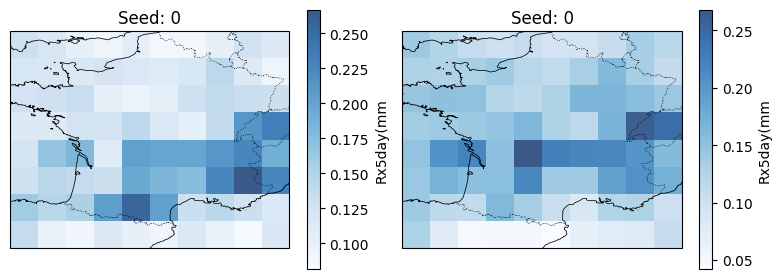
\includegraphics[width=\textwidth]{../images/VAE/vae_decoded_random_maps_seed_zero.png}
            \captionof*{figure}{\scriptsize Cartes synthétiques (VAE)}
        \end{column}
        \begin{column}{0.55\textwidth}
            \centering
            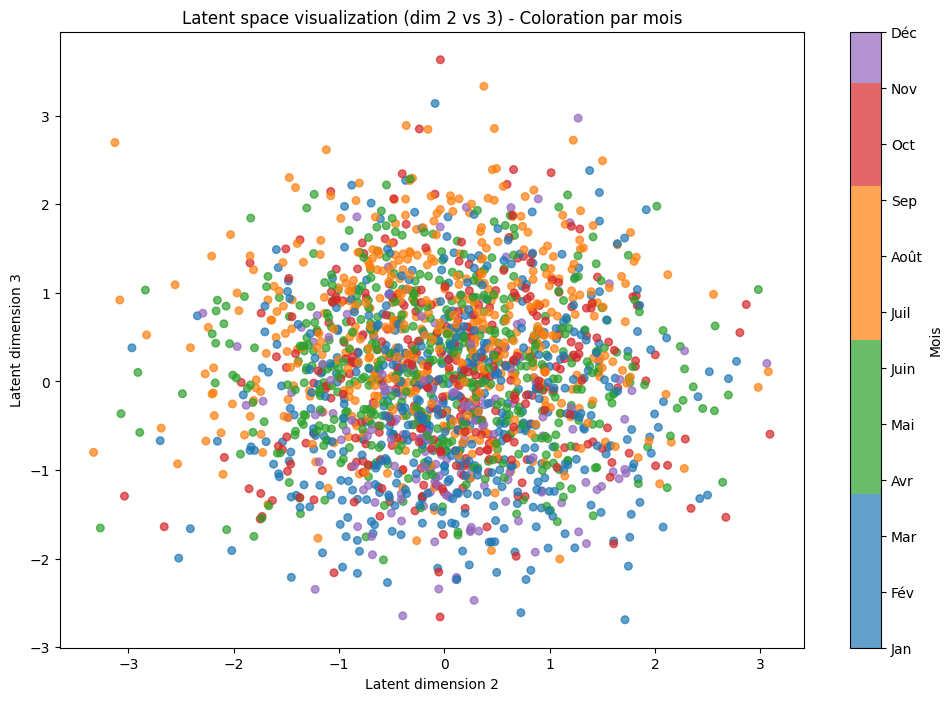
\includegraphics[width=0.8\textwidth]{../images/VAE/vae_latent_space_by_season.png}
            \captionof*{figure}{\scriptsize Espace latent projeté par saison}
            \begin{itemize}
                \item \textbf{Génération} : Cartes cohérentes géographiquement mais intrinsèquement \textbf{floutées/lissées}.
                \item \textbf{Latent} : Chevauchement des saisons normal car des tempêtes d'été et d'automne peuvent partager la même signature spatiale.
            \end{itemize}
        \end{column}
    \end{columns}
\end{frame}

% Slide 9 : GAN
\begin{frame}{Modèles Adversariaux : GAN [4] \& WGAN-GP [5]}
    \textbf{Objectif :} Surmonter le flou du VAE pour générer des contrastes violents (tempêtes).
    \vspace{0.4cm}
    \begin{columns}
        \begin{column}{0.5\textwidth}
            \textbf{GAN classique :}
            \begin{itemize}
                \item Jeu minimax entre Générateur et Discriminateur probabiliste.
                \item \textit{Problème} : Convergence très instable, effondrement de mode fréquent.
            \end{itemize}
        \end{column}
        \begin{column}{0.5\textwidth}
            \textbf{WGAN-GP :}
            \begin{itemize}
                \item Utilise la \textbf{distance de Wasserstein} (Earth Mover's Distance).
                \item Le Discriminateur devient un "Critique" continu.
                \item Régularisation par pénalité de gradient (GP) pour garantir la stabilité.
            \end{itemize}
        \end{column}
    \end{columns}
    \vspace{0.4cm}
    \begin{alertblock}{Le piège de la sparsité}
        La précipitation est dominée par des zéros. Le Discriminateur d'un GAN classique repère instantanément les erreurs de sparsité (ex: pluie diffuse là où il ne devrait rien y avoir), rejetant tout en bloc et \textbf{tuant le gradient} du Générateur.
    \end{alertblock}
\end{frame}

% Slide 10 : Entraînement GAN
\begin{frame}{Entraînement des GANs : Dynamique et Pertes}
    \begin{columns}
        \begin{column}{0.5\textwidth}
            \centering
            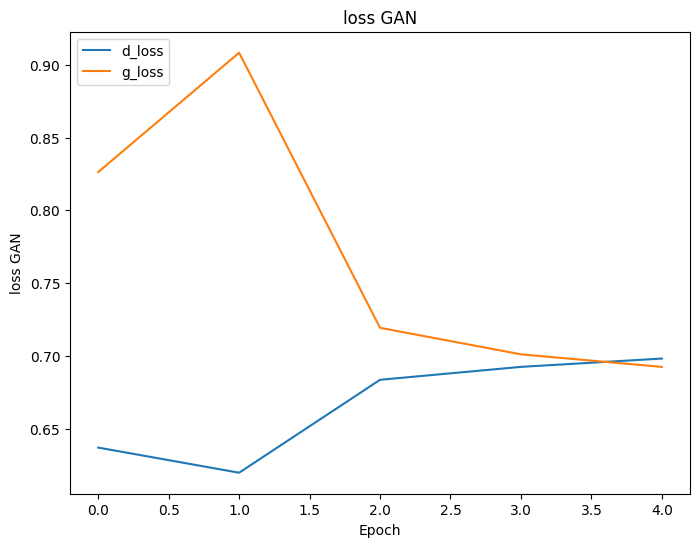
\includegraphics[width=0.95\textwidth]{../images/GAN/gan_training_loss_curve.png}
            \captionof*{figure}{\scriptsize Instabilité du GAN classique (oscillations)}
        \end{column}
        \begin{column}{0.5\textwidth}
            \centering
            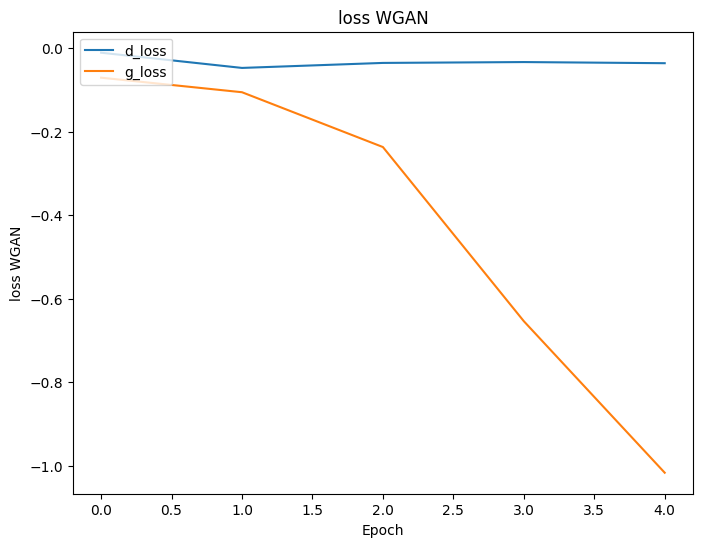
\includegraphics[width=0.95\textwidth]{../images/GAN/wgan_training_loss_curve.png}
            \captionof*{figure}{\scriptsize Dynamique plus lisse du WGAN-GP}
        \end{column}
    \end{columns}
    \vspace{0.4cm}
    \begin{itemize}
        \item La perte de Wasserstein (WGAN-GP) reflète mieux la convergence réelle du modèle et évite le phénomène de mode collapse.
    \end{itemize}
\end{frame}

% Slide 11 : Résultats GAN
\begin{frame}{Résultats : GAN vs WGAN-GP}
    \begin{columns}
        \begin{column}{0.5\textwidth}
            \centering
            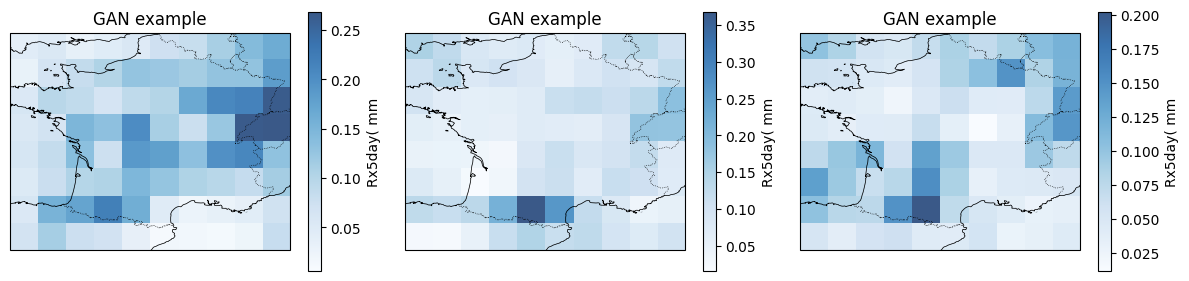
\includegraphics[width=0.9\textwidth]{../images/GAN/gan_final_generated_precipitation_maps.png}
            \captionof*{figure}{\scriptsize Générations GAN classique}
        \end{column}
        \begin{column}{0.5\textwidth}
            \centering
            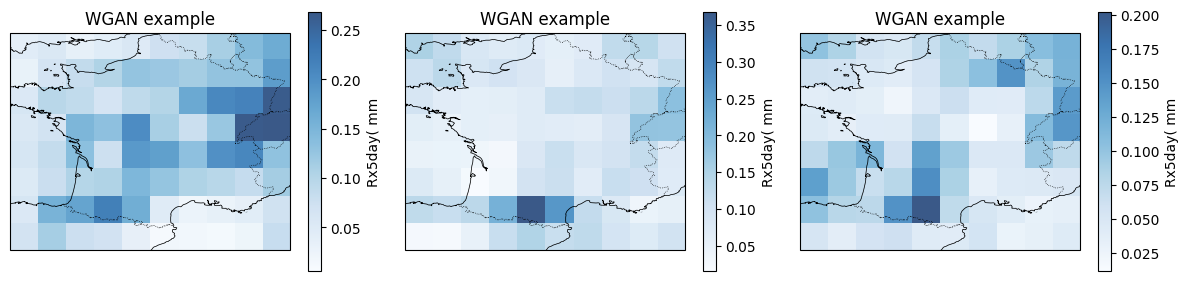
\includegraphics[width=0.9\textwidth]{../images/GAN/wgan_final_generated_precipitation_maps.png}
            \captionof*{figure}{\scriptsize Générations WGAN-GP}
        \end{column}
    \end{columns}
    \vspace{0.3cm}
    \begin{itemize}
        \item Les modèles adversariaux produisent des \textbf{contrastes beaucoup plus abrupts} que le VAE (idéal pour simuler des cellules orageuses locales).
        \item WGAN-GP offre une diversité supérieure au GAN classique, mais souffre encore d'artefacts géométriques en damier (\textit{checkerboard artefacts}).
    \end{itemize}
\end{frame}

% Slide 11 : Bilan
\begin{frame}{Bilan Comparatif des Architectures}
    \begin{table}
        \centering
        \small
        \begin{tabular}{lccc}
            \toprule
            \textbf{Critère} & \textbf{VAE} & \textbf{GAN classique} & \textbf{WGAN-GP} \\
            \midrule
            Stabilité d'entraînement & \textcolor{green!70!black}{Excellente} & \textcolor{red!70!black}{Médiocre} & \textcolor{orange}{Moyenne} \\
            Rendu des contrastes extrêmes & \textcolor{red!70!black}{Faible (Flou)} & \textcolor{green!70!black}{Fort} & \textcolor{green!70!black}{Fort} \\
            Interprétabilité (Latent) & \textcolor{green!70!black}{Oui (Continu)} & \textcolor{red!70!black}{Non} & \textcolor{red!70!black}{Non} \\
            Sensibilité à la sparsité & \textcolor{orange}{Moyenne} & \textcolor{red!70!black}{Très élevée} & \textcolor{orange}{Gérée} \\
            Présence d'artefacts & \textcolor{green!70!black}{Non} & \textcolor{red!70!black}{Oui} & \textcolor{red!70!black}{Oui (Damier)} \\
            \bottomrule
        \end{tabular}
    \end{table}
    \vspace{0.4cm}
    \textbf{Conclusion intermédiaire :} Aucun modèle n'est parfait isolément. Le VAE est le plus robuste pour explorer le climat, mais le GAN est le seul capable d'émuler la brutalité visuelle d'une tempête.
\end{frame}

% Slide 12 : Conclusion
\begin{frame}{Conclusion et Perspectives}
    \textbf{Synthèse des travaux :}
    \begin{itemize}
        \item L'émulation d'extrêmes climatiques (Rx5day) par Deep Learning est possible mais entravée par la distribution asymétrique (queue lourde) des précipitations.
        \item Le réglage minutieux des hyperparamètres (notamment un petit \textit{batch size} pour le VAE) est une condition \textit{sine qua non} pour ne pas lisser les extrêmes.
    \end{itemize}
    \vspace{0.5cm}
    \textbf{Perspectives d'amélioration :}
    \begin{enumerate}
        \item \textbf{Modèles Hybrides :} Développer un modèle \textbf{VAE-GAN} pour allier la stabilité encodée du VAE et la netteté du Critique WGAN.
        \item \textbf{Génération Conditionnelle :} Injecter des variables forçantes (saison, température, altitude) pour diriger la génération (cGAN).
        \item \textbf{Métriques Quantitatives :} Dépasser l'évaluation visuelle via la Distance de Wasserstein empirique et la \textit{Fréchet Inception Distance} (FID) climatique.
    \end{enumerate}
\end{frame}

% Slide 13 : Références
\begin{frame}{Références}
    \begin{thebibliography}{9}
        \setbeamertemplate{bibliography item}[text]
        \bibitem{copernicus}
        [1] Copernicus CDS. \textit{Climate extreme indices from CMIP6 projections}. (2025).
        \bibitem{cmip6}
        [2] Eyring, V. et al. \textit{Overview of the CMIP6 experimental design}. GMD, (2016).
        \bibitem{vae}
        [3] Kingma, D. P., \& Welling, M. \textit{Auto-Encoding Variational Bayes}. ICLR, (2014).
        \bibitem{gan}
        [4] Goodfellow, I. et al. \textit{Generative Adversarial Nets}. NeurIPS, (2014).
        \bibitem{wgan}
        [5] Gulrajani, I. et al. \textit{Improved Training of Wasserstein GANs}. NeurIPS, (2017).
    \end{thebibliography}
\end{frame}

% ==========================================
% ANNEXES
% ==========================================
\appendix

\begin{frame}[noframenumbering]{Annexe : Espace Latent VAE (Détails)}
    \centering
    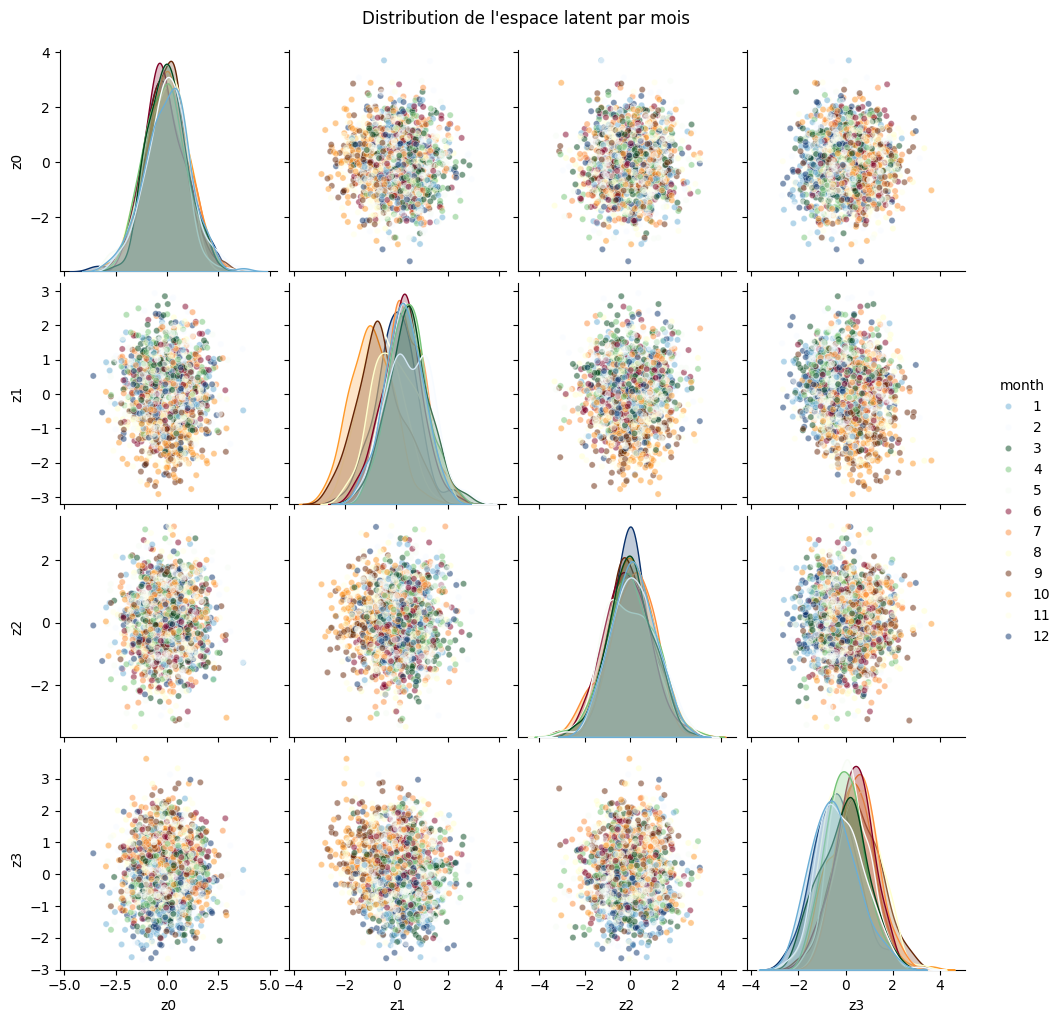
\includegraphics[width=0.6\textwidth]{../images/VAE/vae_latent_pairplot_by_season.png}
    \captionof*{figure}{\scriptsize Pairplot des 8 dimensions latentes du VAE, colorées par saison.}
\end{frame}

\end{document}